% Cover letter: Stage IoT (Job ID 2463, Roma / Milano), BIP
% CV: Sections/cv_iot_engineer.tex -> cv_gen/cv_giovanni_tauro-bip.pdf
% Letter in Italian (the posting is in Italian). babel-italian is not installed here,
% so hyphenation is switched off instead of using English patterns on Italian words.
\documentclass[11pt,a4paper,sans]{moderncv}
% Shared preamble and header for the cover letters.
% One main file per application: cl_<company>.tex, built to
% cv_gen/coverletter_giovanni_tauro-<company>.pdf next to cv_giovanni_tauro-<company>.pdf.
% Paths (cl_gen/..., Pictures/...) are relative to the project root, as in the CV (see .latexmkrc).

\moderncvstyle{classic}
\moderncvcolor{blue}

\usepackage[scale=0.80]{geometry}
\setlength{\footskip}{136.00005pt}

\usepackage{fontawesome5}
% hyperref is loaded by moderncv itself; loading it here causes an option clash
\usepackage{xcolor}
\usepackage{graphicx}
\ifxetexorluatex
  \usepackage{fontspec}
  \usepackage{unicode-math}
  \defaultfontfeatures{Ligatures=TeX}
  \setmainfont{Latin Modern Roman}
  \setsansfont{Latin Modern Sans}
  \setmonofont{Latin Modern Mono}
  \setmathfont{Latin Modern Math}
\else
  \usepackage[T1]{fontenc}
  \usepackage{lmodern}
\fi

\usepackage[english]{babel}

% used for the PDF title and the letter closing; the visible header is \clheader below
\name{Giovanni}{Tauro}

% Header: #1 = headline under the name (same as the headline of the matching CV)
\newcommand{\clheader}[1]{%
\noindent
\begin{minipage}[c]{0.74\textwidth}
    {\Huge \textbf{Giovanni Tauro}}\\[-0.2em]
    {\small #1}\\[0.3em]

    \footnotesize
    \faMapMarker*~
    \href{https://www.google.com/maps/search/?api=1&query=Lecco+23900+Italy}
    {\color{blue}Bari-Lecco, Italy}
    \quad
    \faPhone*~
    \href{https://wa.me/393279437161}
    {\color{blue}+39 3279437161}
    \quad
    \faEnvelope~
    \href{mailto:giovanni.taurodi@gmail.com}
    {\color{blue}giovanni.taurodi@gmail.com}
    \\[-0.1em]

    \faLinkedin~
    \href{https://www.linkedin.com/in/giovanni-tauro-gt/}
    {\color{blue}LinkedIn}
    \quad
    \faGithub~
    \href{https://github.com/jotades}
    {\color{blue}GitHub}
    \quad
    \faGraduationCap~
    \href{https://scholar.google.com/citations?user=BS0aVGgAAAAJ&hl=it}
    {\color{blue}Scholar}
    \quad
    \faFilePdf~
    \href{https://www.notion.so/Giovanni-Tauro-2a7901d92f3a800b892af425c5875c6a}
    {\color{blue}Portfolio}
    \quad
    \faCubes~
    \href{https://grabcad.com/giovanni.tauro-3}
    {\color{blue}GrabCAD}

\end{minipage}
\hfill
\begin{minipage}[c]{0.18\textwidth}
    \raggedleft
    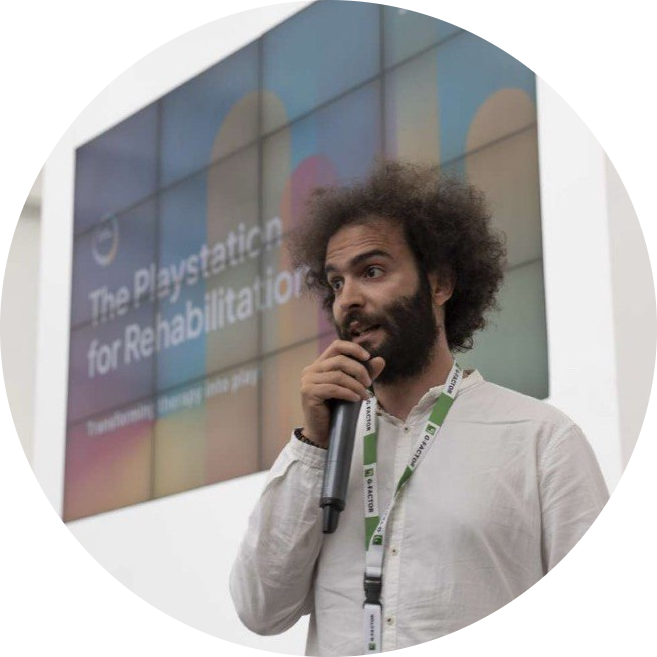
\includegraphics[width=2.8cm]{Pictures/Giovanni_pitch}
\end{minipage}
\vspace{0.1em}
}

\makeatletter
% the sender details are already in \clheader, so skip moderncv's own block
\@detailsfalse
% closing phrase, signature, name
\renewcommand*{\makeletterclosing}{%
  \@closing\\[0.6em]%
  
\includegraphics[height=1.2cm]{Pictures/sign_gt.jpg}\\[0.2em]%
  {\bfseries\@firstname~\@lastname}}
\makeatother


\begin{document}
\hyphenpenalty=10000 \exhyphenpenalty=10000 \emergencystretch=3em

\clheader{R\&D Engineer, PhD Candidate | Embedded Systems \& IoT}

\recipient{Team Talent Acquisition}{BIP}
\date{13 ottobre 2026}
\opening{Gentile team di selezione,}
\closing{Cordiali saluti,}
\makelettertitle

vi scrivo per candidarmi alla posizione Stage IoT (Job ID 2463). Sono R\&D engineer al CNR-STIIMA e dottorando all'Università di Bologna, e negli ultimi anni mi sono occupato soprattutto di un progetto: OmniTrack.

OmniTrack è nato da un'idea semplice: aiutare una persona a orientarsi in una stanza guidandola verso un punto con segnali visivi, sonori e aptici che cambiano man mano che si avvicina, un po' come nel gioco acqua e fuoco. Da quell'idea ho seguito tutto il percorso: la scelta dei componenti, i primi prototipi, il firmware in C++ dei moduli ESP32 che misurano le distanze in UWB, il collegamento via Bluetooth a un sistema ROS 2 su Linux che calcola la posizione, e la logica che regola il feedback in base alla distanza dall'obiettivo.

Poi è arrivata la parte che considero più importante, cioè capire se lo strumento funzionava davvero. Ho misurato l'errore di localizzazione, l'ho ridotto con una calibrazione e un filtraggio dei dati, e ho portato il sistema fuori dal laboratorio in uno studio con 16 partecipanti non vedenti. Il lavoro è descritto nell'articolo \href{https://www.frontiersin.org/journals/communications-and-networks/articles/10.3389/frcmn.2026.1829998/abstract}{\color{blue}\textit{OmniTrack: A Multimodal IoT System for Indoor Localization and Feedback to Support Perceptual--Motor Skill Training}} (Frontiers in Communications and Networks, 2026), di cui sono primo autore.

Questo percorso mi ha insegnato a portare un sistema IoT dall'idea alla validazione, ma sempre alla scala di un prototipo di ricerca: pochi dispositivi, una stanza, un gruppo di utenti. Quello che mi manca, e che cerco in BIP, è imparare a scalare: come si progettano sistemi e software pensati per molti dispositivi, per la produzione e per clienti con esigenze diverse. Mi candido per questo, e perché nell'annuncio ritrovo le attività che mi piace fare, dal bring-up di una scheda all'integrazione del software.

Porto con me anche l'abitudine a lavorare con persone non tecniche. Sia al CNR sia in Rehabilia Technologies, la startup di cui sono co-fondatore, ho definito i requisiti dei dispositivi insieme a clinici e utenti.

Sarei felice di raccontarvi di più in un colloquio.

\makeletterclosing

\end{document}
